\chapter{Decision-making}

Everyday, humans and non-humans make hundreds of \glspl{decision}, each of them leading to a \gls{choice} between several possible alternatives. Some of these decisions are trivial: for example, choosing which socks to wear when dressing up. Others imply higher stakes: for example, deciding to embark oneself on a PhD.

\Gls{decision-making} is one of the main aspects of cognition. Its study spans such varied scientific fields as psychology, neuroscience, economics, statistics and political science. Despite the immense variety of contexts and applications, most decisions share common elements including deliberation and commitment \cite{goldNeuralBasisDecision2007}. In the following chapters, we study the main properties of decisions and review some computational models of decision-making.

\section{Properties of decisions}

A decision is a deliberative process resulting in the commitment to a categorical proposition \cite{goldNeuralBasisDecision2007}. An often used analogy is a jury weighting the available evidence before settling on a verdict.

The following sections describe some characteristical traits of decisions.

\subsection{Decision types}

Some decisions involve discriminating between sensory stimuli. Some examples of experimental scenarios associated to such perceptual decisions are Stroop tasks (naming the ink color of a colored word with a mismatch between ink color and word), \acrlong{rdm} tasks (assessing the main motion of a dot cloud, Figure \ref{figure:rdm}) or faint sound detection. In that case, the alternatives are typically well-defined and mutually exclusive (e.g., "sound present" vs. "sound absent").

\begin{figure}[ht]
    \centering
    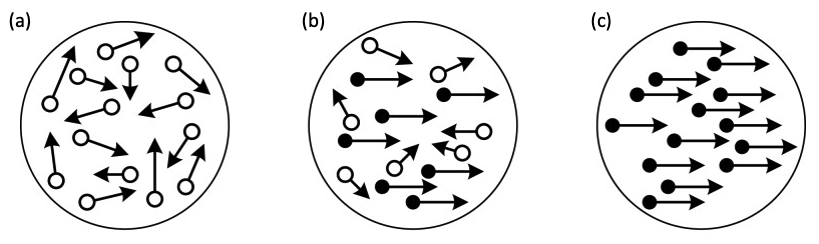
\includegraphics[width=\textwidth]{random_dot_motion.png}
    \caption[Examples of Random Dot Motion tasks]{Examples of Random Dot Motion tasks with various movement coherence. \textbf{(a)} Coherence = $0$: dots are moving randomly. \textbf{(b)} Coherence = $0.5$: half of dots are moving to the right. \textbf{(c)} Coherence = $1$: all dots are moving to the right.}
    \label{figure:rdm}
\end{figure}

Other decisions require choosing between alternatives based on subjective preferences or expected rewards. Examples of experimental scenarios associated to such value-based decisions are \acrlong{mab} problems, in which a decision-maker iteratively selects one of multiple fixed choices (e.g., arms or actions) in order to maximize a cumulative reward.

\subsection{Time course}

All decisions are made under a form of time pressure \cite{forstmannSequentialSamplingModels2016}: one simply cannot take hours to ponder over his or her socks collection, or wait indefinitely before accepting a PhD offering. A decision takes place at the end of a deliberation phase, in which available information is acquired and processed by the decision-maker. Many decisions are based on information that unfolds over time: for example, tasting wine before recognizing its grape variety. Even when all information is immediately available (for example, a chessboard observed by a player before choosing his or her next move), it generally has to be treated sequentially, reflecting the inability of the decision-maker's cognitive system to process all information simultaneously. Thus, the sequential nature of the decision process is a fundamental property of biological nervous systems \cite{forstmannSequentialSamplingModels2016}.

More formally, a decision can be envisioned as the mapping from a stimulus to a response. Time between stimulus and response execution is called \acrfull{rt} \cite{forstmannSequentialSamplingModels2016}, \cite{myersPracticalIntroductionUsing2022}. It can be decomposed into three parts: the time required to encode the stimulus ($Te$), the time to make a decision ($Td$), and the time to execute the selected response ($Tr$).

$$RT = T_e+T_d+T_r$$

\begin{figure}[ht]
    \centering
    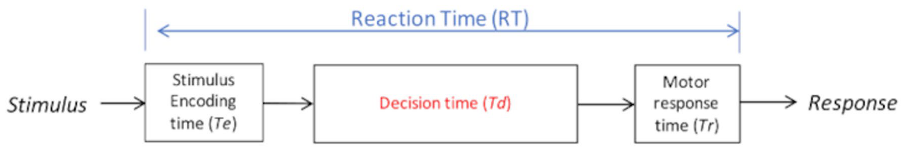
\includegraphics[width=\textwidth]{myersPracticalIntroductionUsing2022_1.png}
    \caption[Decomposition of \acrlong{rt} for a decision]{The \acrfull{rt} is assumed to reflect the time required to encode the stimulus ($Te$), the time to make a decision ($Td$), and the time to execute the selected motor response ($Tr$). The encoding and motor response time are typically combined into a single parameter, $Ter$, representing non-decision time. Adapted from \cite{myersPracticalIntroductionUsing2022}}
\end{figure}

\subsection{\acrlong{sat}}

A related criterion is the possibility of objectively evaluating the decision outcome. Some decisions have correct or optimal answers, to which the chosen alternatives can be compared in order to compute evaluation metrics like \gls{accuracy}. This is typically the case for perceptual decisions, for which the expected results are controlled by the experimenter. On the other hand, some value-based decisions cannot be objectively evaluated: for example, picking one's favorite color.

For decisions whose outcome can be assessed, the balance between \acrshort{rt} and accuracy is called the \acrfull{sat}. This ubiquitous aspect of decision-making has been a phenomenon of interest in behavioral science for a long time \cite{heitzSpeedaccuracyTradeoffHistory2014}. The \acrshort{sat} is at least partially under the decision-maker's control: a faster decisions can ne taken at the expense of an higher error rate, and vice-versa \cite{ratcliffDiffusionDecisionModel2016}. As such, one must not only consider accuracy and speed, but also the interaction between them when studying decisions \cite{myersPracticalIntroductionUsing2022}.

\subsection{Uncertainty}

\Gls{uncertainty} (or incertitude) is an inherent part of decision-making processes. Generally speaking, it characterizes situations involving imperfect, noisy or unknown information. In the narrower context of decision-making, \gls{uncertainty} refers to the variability in the representation of information before a decision is taken \cite{mamassianConfidenceForcedChoiceOther2020}.

\Gls{uncertainty} is inherent to all stages of neural computation. The brain can, and likely does, track uncertainty in a whole host of quantities \cite{flemingMetacognitionConfidenceReview}. For example, driving one's car requires processing different visual, auditory and vestibular inputs (each corrupted by noise) in order to adapt to a continuous stream of not-so-predictable external events (a child or an animal crossing the street, the car in front of yours breaking suddenly, and so on) \cite{pougetConfidenceCertaintyDistinct2016}.

Uncertainties can be further classified into two categories \cite{yuUncertaintyNeuromodulationAttention2005}. Expected uncertainty, also called stochasticity, represents "known unknows". It arises from known unreliabilities of predictive relationships within a familiar environment. On the other hand, unexpected uncertainty, also called volatility, represents "unknown unknows". It is due to impredictable changes in the environment. For example, the decision whether to bring un umbrella in the morning requires evaluating the possibility of a misforecast by one's usual weather prediction system. Occasional errors (expected uncertainty) would reflect the noisy nature of the process, while a substantial drop in forecast reliability (unexpected uncertainty) would induce a change in the weather prediction model. For decision-makers, disentangling and assessing uncertainty types is key to an efficient behavior. \todo{Faire le lien avec aleatoric/epistemic uncertainty?}

\section{Models of the decision process}

One approach to understanding decision-making is through computational modeling. Many solutions have been proposed to describe the decision process, ranging from detailed models of neural circuits to abstract psychological models of behaviour \cite{bogaczOptimalDecisionmakingTheories2007}, \cite{teodorescuDisentanglingDecisionModels2013}. The following sections review several prominent models of decision-making.

We start by studying solutions for modeling a single decision. When only one piece of information is available, \acrfull{sdt} is the framework of reference. When multiple pieces are available over time, extensions of \acrshort{sdt} account for the sequential integration of information by the decision-maker. They are called \acrlong{eam}s (\acrshort{eam}s).

Another important scenario of decision-making is when decisions are followed by rewards and produce learning effects. A dedicated class of models combines evidence accumulation and \acrfull{rl} to describe these mutually influential processes.

\subsection{Conceptual overview}

A decision can be thought of as a form of statistical inference \cite{goldNeuralBasisDecision2007}. A decision-maker must select among $n \in \mathbb{N^{+}}$ competing hypotheses denoted $h_i$, with $i \in [1,n]$ and $n \ge 2$. For example, a jury may have to rate a defendant on a scale of $1$ (\textit{most certainly guilty}) to $5$ (\textit{most certainly innocent}).

The probability $P(h_i)$, called \textit{prior}, refers to the probability that $h_i$ is true before obtaining any information about it. In the courtroom analogy, these priors correspond to prejudices that can bias jurors’ judgments Decisions are informed by data, often called \textit{evidence} and denoted $e$. Each evidence bears on a particular hypothesis $h_i$. For example, a DNA sample collection can be used as evidence for either supporting or opposing the hypothesis that a person was present at a crime scene. Each possible outcome can be attributed a value, denoted $v$. Value reflects either the subjective costs (for example, wasted time or consumed resources) or benefits (received rewards) derived from a choice.

All sources of priors, evidence and value are integrated into a conceptual entity called a \acrfull{dv} \cite{goldNeuralBasisDecision2007}. A decision rule determines how and when this quantity is interpreted to commit to a particular alternative $H_i$ (the choice associated with hypothesis $h_i$). In the previous example, the rule causes the jury to declare, “we have a verdict.” A simple rule is to place a criterion value on it: the decision is made if (or when) the \acrshort{dv} reaches this threshold.

\subsection{Modeling a binary decision}

\subsubsection{\acrlong{sdt}}

\acrfull{sdt} is a framework for analysing \gls{decision-making} in the presence of uncertainty. Originally developped in the mid-20th century to assess how faithfully a radar operator was able to separate signal (enemy missiles or planes) from noise (random interferences or electronical artefacts), it has applications in many fields: psychology, diagnostics, quality control, etc \cite{green1966signal}.

\acrshort{sdt} measures the ability of a decision-maker to discriminate two possible stimulus types, generally called \textit{signal} and \textit{noise}, from one piece of information \cite{stanislawCalculationSignalDetection1999}. A simple example of using \acrshort{sdt} in experimental psychology is when testing the ability of a subject to detect a short tone (signal) in a background of white noise. Another example could be a memory recognition test: assess stimuli items as already seen (signal) or new (noise).

In a binary task, also called a \acrfull{2afc}, signals are either present or absent in the stimuli. The response given by the subject for each trial can be sorted in one of four categories (Table \ref{table:1}).

\begin{table}[h!]
    \centering
    \begin{tabular}{ ||c||c|c|| }
        \hline
        Signal  & Response: "absent"        & Response: "present" \\
        \hline\hline
        Absent  & Correct Rejections ($TN$) & False Alarms ($FP$) \\
        \hline
        Present & Misses ($FN$)             & Hits ($TP$)         \\
        \hline
    \end{tabular}
    \caption{Categorization of responses in a binary decision task.}
    \label{table:1}
\end{table}

The \textit{hit rate} (the probability of responding yes on signal trials), also called \acrfull{tpr}, and the \acrfull{fpr}, the probability of responding yes on noise trials, are two metrics that describe results.

$$\text{TPR} = \frac{TP}{TP + FN}$$

$$\text{FPR} = \frac{FP}{TN+FP}$$

\acrshort{sdt} represents a decision as a comparison between a \acrfull{dv}, directly derived from a single piece of evidence caused by a stimulus, and a criterion (the threshold between the “noise” and “signal” responses) set by the decision-maker. This model can be applied to decision tasks in which a single stimulus is presented on each trial. Depending on the task, the \acrshort{dv} might be observable, or available only to the decision-maker. For example, the \acrshort{dv} may be the loudness experienced during each trial in an auditory perception study, or the feeling of familiarity associated with each stimulus item in a memory study.

The evidence $e$ is affected by factors both external (such as variations in stimulus strength) and internal (such as neural noise or limited resources). Its magnitude differs depending on the underlying stimulus: it will have a range of different values across signal trials and a range of different values across noise trials. Thus, $e$ can be considered a random variable. Its distribution across signal trials is the \textit{signal distribution}, whereas the corresponding distribution for noise trials is the \textit{noise distribution}. These conditionalized distributions define the likelihoods $P(e|h_i)$ (value of $e$ in the presence/absence of signal). In the general case, the two distributions will overlap, reflecting the task difficulty. The decision requires the construction of a \acrlong{dv} from $e$. For binary decisions, the \acrshort{dv} is typically related to the ratio of the likelihoods of $h_1$ (signal present) and $h_2$ (no signal) given $e$ (Figure \ref{figure:sdt}).

$$DV(e) = \frac{P(e|h_1)}{P(e|h_2)}$$

\begin{figure}[ht]
    \centering
    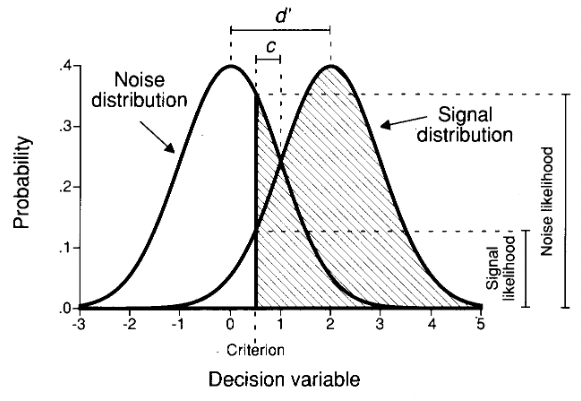
\includegraphics[scale=0.6]{stanislawCalculationSignalDetection1999_1.png}
    \caption[\acrlong{sdt}: graphical formalism]{\acrlong{sdt}: hypothetical probability density functions (likelihoods) for noise and signal distributions of the evidence. The distribution has a mean of 0 and a standard deviation of 1 on noise trials. On signal trials, the mean is higher ($M = 2$), but the standard deviation is unchanged. A \textit{yes} response is made for trials in which the \acrlong{dv} exceeds the criterion, located at $0.5$; these trials lie in the shaded region of the two distributions. The \acrlong{tpr} equals the proportion ofthe signal distribution that exceeds the criterion ($\acrshort{tpr} = 0.9332$). The \acrlong{fpr} equals the proportion of the noise distribution that exceeds the criterion ($\acrshort{fpr} = 0.3085$). Response bias can be quantified by either the likelihoods ratio $\beta$ at the criterion location ($\beta = \frac{0.1295}{0.3521} = 0.37$), or the distance $c$ between the criterion and the neutral point ($c = -0.5$). Both distributions are normal and of equal variance, so $d'$ is a bias-free measure of sensibility ($d'=2$). Adapted from \cite{myersPracticalIntroductionUsing2022}}
    \label{figure:sdt}
\end{figure}

\acrlong{sdt}'s main virtue is its ability to disentangle two factors in a decision process: the tendency towards responding \textit{yes} regarless of the stimulus, called \textit{bias}, and the ability to distinguish signal from noise, called \gls{sensitivity}. For example, industry quality-control inspectors often detect fewer faulty items as their work shift progresses. \Acrshort{sdt} demonstrated that this declining hit rate usually results from a change in response bias rather than a declining \gls{sensitivity}.

Bias is determined by the criterion location. A lower (liberal) criterion biases the decision-maker towards \textit{yes} responses, while a higher (conservative) value has the opposite effect. Bias can be quantified using either the ratio of the likelihoods for the two distributions at the criterion location (denoted $\beta$), or the distance between the criterion and the neutral point where distributions cross and neither response is favored, denoted $c$ and measured in standard deviation units.

\Gls{sensitivity} is determined by the degree of overlap between the noise and signal distributions. It is related to the distance between the means of the noise and signal distributions. One possible measure of \gls{sensitivity} is $d'$, which is the distance between the means in standard deviation units. Two assumptions must be met for $d'$ to be a bias-free measure of sensibility: the noise and signal distributions must be normal (Gaussian) and have the same variance (standard deviation). It can be obtained using the inverse cumulative distribution function, which computes the standard score (z-score) associated to a probability \cite{stanislawCalculationSignalDetection1999}.

Another possible measure of sensibility uses the \acrfull{roc} curve, which plots the \acrlong{tpr} as a function of the \acrlong{fpr} for all possible values of the decision criterion. Computing the \acrfull{auroc} is a non-parametric way to assess \gls{sensitivity} independently of bias that is free from the equal-variance Gaussian assumptions needed for $d'$ to be bias-free \cite{flemingHowMeasureMetacognition2014} (Figure \ref{figure:roc_curves}).

\begin{figure}[ht]
    \centering
    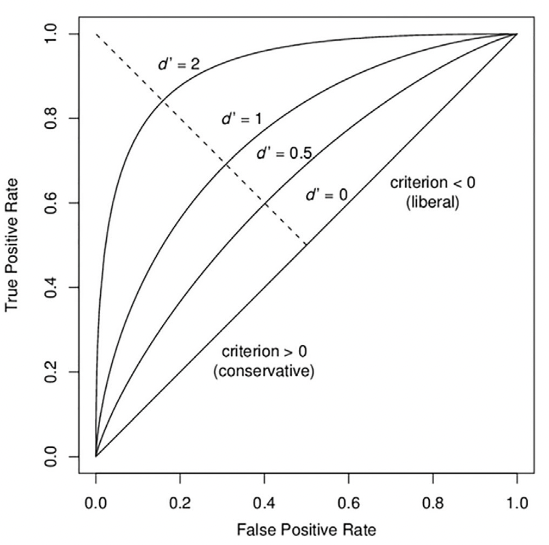
\includegraphics[scale=0.5]{michelConfidenceConsciousnessResearch2023_1.png}
    \caption[\acrlong{sdt}: \acrshort{roc} curves]{\acrlong{sdt}: \acrshort{roc} curves connecting locations with constant $d'$. The major diagonal is called the “chance line” since the \acrlong{tpr} and \acrlong{fpr} are equal, meaning that the subject is performing at chance level. A conservative criterion decreases both \acrshort{tpr} and \acrshort{fpr}, and a liberal criterion increases them. Using the \acrfull{auroc} is a way to assess \gls{sensitivity} independently of the response criterion. Adapted from \cite{michelConfidenceConsciousnessResearch2023}}
    \label{figure:roc_curves}
\end{figure}

\subsubsection{\acrlong{ssm}s}

For its many qualities, \acrlong{sdt} is silent on decision time. Another class of decision-making models assume that the \acrshort{dv} is constructed from multiple pieces of evidence integrated over time. The process stops when a threshold is reached, which triggers the decision. This approach, called \textit{\gls{sequential sampling}} or \textit{sequential analysis}, allows studying the relationship between accuracy and the time needed to take a decision. Different approaches to sequential sampling coexist. Models differ according to the number of \acrlong{dv}s, and whether these are independent, correlated or subject to non-linear operations like decay or mutual inhibition (Figure \ref{figure:sequential_sampling} \todo{Ajouter la description des modèles hybrides}). Models belonging to this family are called \acrlong{ssm}s or \acrlong{eam}s.

\subsubsection{\acrlong{sprt}}

A well-known form of sequential sampling for binary decisions is the \acrfull{sprt}. It uses a single \acrlong{dv} which is constructed from $n$ multiple, independent pieces of evidence $e_1, e_2, \dots, e_n$ as the logarithm of the likelihood ratio between the two hypotheses $h_1$ and $h_2$.

$$DV(e_1, \dots, e_n) = \sum_{i=1}^n log_e \frac{P(e_i|h_1)}{P(e_i|h_2)} = \sum_{i=1}^n w_i$$

The $w_i, i \in [1,n]$ term represents the weight of the $i$th evidence in favor of the $h_1$ hypothesis. The \Acrshort{dv} is updated with new pieces of evidence until reaching a criterion. It is optimal in the sense that it achieves the fastest mean decision time for a given accuracy \cite{bogaczOptimalDecisionmakingTheories2007}. As an example, consider two coins placed in a bag: one is fair (50/50 chance of obtaining heads or tails when tossing it), the other not (60/40). One of the coins is drawn from the bag: is it a trick ($h_1$) or a fair ($h_2$) coin? And how many tosses are needed for this decision? To answer these questions, each toss result $e_i$ is converted to a weight of evidence $w_i$.

$$\forall i \in[1,n], w_i=
    \begin{cases}
        \log_e \frac{P(e_{heads}|h_1)}{P(e_{heads}|h_2)} = \log_e \frac{0.6}{0.5} = 0.182  & \text{if toss gives "heads"} \\
        \log_e \frac{P(e_{tails}|h_1)}{P(e_{tails}|h_2)} = \log_e \frac{0.4}{0.5} = -0.223 & \text{if toss gives "tails"}
    \end{cases}$$

Let $\alpha$ be the probability that a fair coin will be misidentified and $\beta$ the probability that a trick coin will be misidentified. The \acrshort{sprt} prescribes that the answer should be "trick" if at any moment, $DV \ge \frac{1-\alpha}{\alpha}$ and "fair" if $DV \le \frac{\beta}{1-\beta}$. \todo{Vérifier les formules pour les bornes du SPRT}. Otherwise, more evidence should be obtained. For example, if $\alpha = \beta = 0.05$, a decision should be made if $|DV| \ge \log_e(19)$.

\begin{figure}[ht]
    \centering
    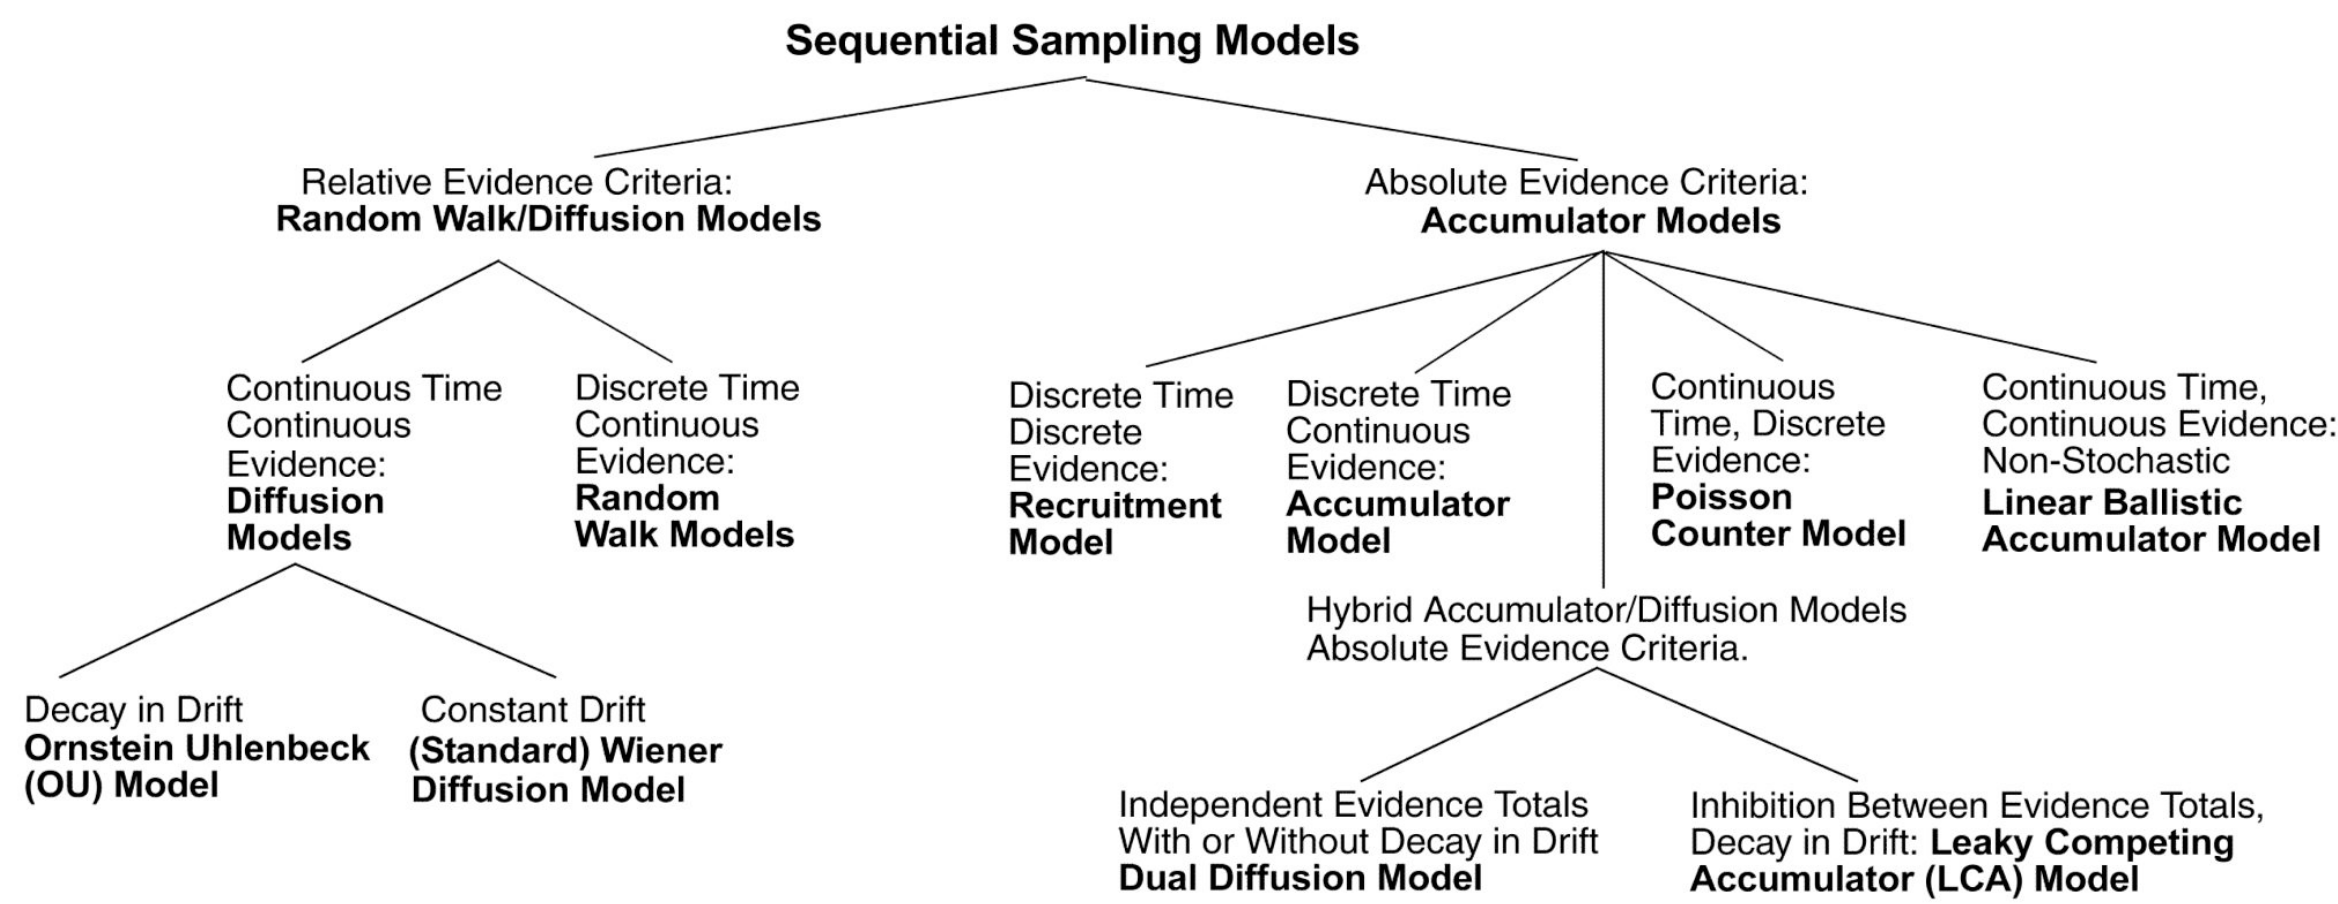
\includegraphics[width=\textwidth,height=\textheight,keepaspectratio]{ratcliffDiffusionDecisionModel2016_1.png}
    \caption[The sequential sampling model family]{The sequential sampling model family. Accumulator models, also known as \textit{race models}, have several \acrlong{dv}s (typically one per possible choice) and an absolute evidence response rule (one threshold for each \acrshort{dv}). Random walk/diffusion models use a relative evidence rule: a decision is made as soon as the difference in integrated evidence reaches a predefined threshold. When there are two alternatives and the \acrshort{dv}s are inversely correlated, a race model is nearly identical to a random walk. Adapted from \cite{ratcliffDiffusionDecisionModel2016}}.
    \label{figure:sequential_sampling}
\end{figure}

\subsubsection{\acrlong{ddm}}

Another prominent model of the decision-making process id the \acrfull{ddm}, also called Drift Diffusion Model \cite{ratcliffDiffusionDecisionModel2008}. Originally designed in the 1970’s, it is a sequential sampling model for binary choices in continuous environments. The \acrshort{ddm} assumes that a decision is based on the accumulation of noisy evidence in a \acrlong{dv}, commencing at a starting point and terminating at one of the two decision thresholds that are associated with each of the alternatives (Figure \ref{figure:ddm}).

\begin{figure}[ht]
    \centering
    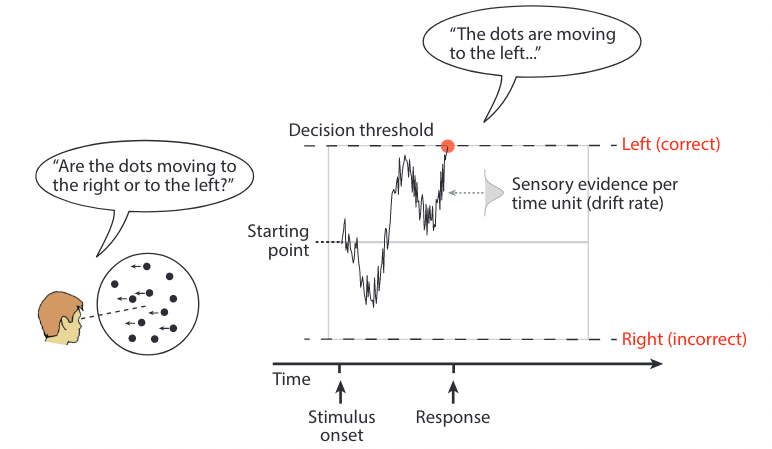
\includegraphics[width=\textwidth,height=\textheight,keepaspectratio]{forstmannSequentialSamplingModels2016_1.png}
    \caption[The \acrlong{ddm}]{Schematic representation of the \acrlong{ddm} on a perceptual discrimination task (\acrlong{rdm}). Evidence is accumulated over time until the threshold associated with the "left" response is crossed. As the input which constitutes the evidence is noisy, the accumulation process is stochastic, mimicking a random walk or the Brownian motion of physical particles. Adapted from \cite{forstmannSequentialSamplingModels2016}.}
    \label{figure:ddm}
\end{figure}

In its canonical form, the \acrshort{ddm} has four parameters. The starting point of evidence accumulation, denoted $z$, represents the a priori bias favoring one of the two alternatives. In an unbiased setting, $z=0$. The decision boundaries are symmetrically described by a parameter denoted $a$, which implements the \acrlong{sat}: increasing $a$ results in fewer errors but also slower responses. The average amount of accumulated evidence per unit of time (i.e. the average speed of evidence accumulation) is called the \textit{drift rate} and denoted $v$. It is an index of task difficulty of subject ability. Lastly, non-decision time $T_{er}$ measures the time needed for peripheral processes such as stimulus encoding and motor response. athematically speaking, the \Acrshort{ddm} assumes that evidence accumulation is governed by the following equation:

$$dx = vdt + sW$$

$x$ represents the accumulated evidence and $dt$ the time unit (when $dt = 0$, the integration process is continuous in time). $s$ is the standard deviation of the within-trial accumulation white noise $W$.

The \acrlong{ddm} is being used by a growing body of literature to elucidate the cognitive processes of decision-making. From a behavioral standpoint, \Acrshort{ddm}-based studies showed that older adults had slower non-decision times and set wider boundaries, but their drift rates were not always lower than those of young adults. \Acrshort{ddm}-based analyses demonstrated that drift rate varied with IQ, but boundary separation and nondecision time did not. Sleep deprivation and alcohol consumption have been linked to a drift rate, but have either small or no effect on boundary separation and non-decision time. From a neuroscience standpoint, studies use the \acrshort{ddm} as inspiration to interpret neuron firing rates in monkeys as evidence accumulation until a threshold is reached \cite{GOLD200110}. Others correlate parameter estimates from \Acrshort{ddm} models to the blood-oxygen-level dependent signal obtained from fMRI experiments in perceptual decision-making. The initial model has been extended to account for specific behavioral patterns like the difference in \acrlong{rt} between correct and error responses \cite{ratcliffDiffusionDecisionModel2008}, or post-deciaional change of mind by the decision-maker \cite{resulajChangesMindDecisionmaking2009}.

\subsection{Handling multiple choices}

\subsubsection{\acrlong{msprt}}

\subsubsection{\acrlong{lca}}

\subsubsection{\acrlong{lba}}

The \acrfull{lba} is a model of decision-making using one \acrlong{dv} per alternative \cite{brownSimplestCompleteModel2008}. Compared to diffusion-based models like the \acrshort{ddm} or the \acrshort{lca}, the \acrshort{lba} makes several simplificative assumptions. First of all, instead of being stochastic by adding some within-trial variability, evidence accumulation is linear. Secondly, all \acrshort{dv}s are independant and not subject to any decay or inhibition mechanism (Figure \ref{figure:lba}). It integrates two sources of inter-trial variability: the starting points for evidence accumulators are random values drawn from a uniform distribution, and the drift rates are drawn from normal distributions with specific means and a common standard deviation. The model takes its name from the fact that the future trajectory of each \acrshort{dv} is fully determined by its initial conditions, corresponding to the notion of ballistics in Newtonian mechanisms.

\begin{figure}[ht]
    \centering
    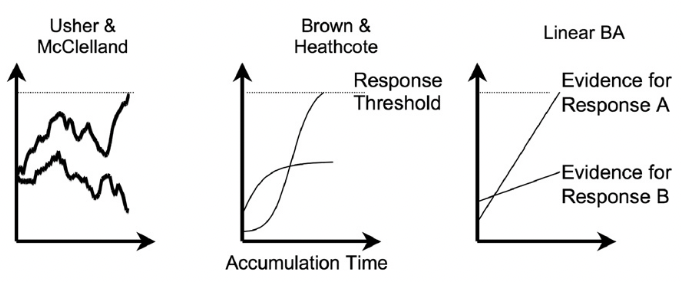
\includegraphics[width=\textwidth,height=\textheight,keepaspectratio]{brownSimplestCompleteModel2008_1.png}
    \caption[The \acrlong{lba}]{Schematic illustration of the differences between the \acrshort{lca} (left). the ballistic accumulator (center) and the \acrshort{lba} (right). The first model uses within-trial stochastic evidence accumulation, decay and mutual inhibition between \Acrlong{dv}s. The second one omits stochastic mechanisms. The third one also drops decay and response competition. Adapted from \cite{brownSimplestCompleteModel2008}.}
    \label{figure:lba}
\end{figure}

Despite these simplifications, the \acrshort{lba} is able to account for the most important experimental results related to decision-making, including the \acrshort{rt} distribution shape, the \acrlong{sat} and the relative speed of correct vs. incorrect responses. \todo{Expliquer qqpart les vitesses relatives des décisions correctes vs. incorrectess}

\subsubsection{\acrlong{alba}}

\todo{Ajouter les modèles RD et ARD ?}

\subsection{Integrating learning effects}